\section{Data, models and storage scheduling}
\label{ch1:sec:data-and-network-models}

In this section the used power data is presented first.
Then the network model, from which all aforementioned key network parameters are extracted, and the battery model are explained.
In the end, the scheduling procedure is detailed.

\subsection{Load profiles}

\nomenclature[I]{$s_\text{net}(t)$}{Apparent network load at time $t$, where $s_\text{net}(t) \in \mathbb{C}$ (Chapter \ref{ch1})}
\nomenclature[I]{$s_{\text{load},i}(t)$}{Apparent load power for load $i$ at time $t$, where $\textbf{s}_\text{load}(t) = (s_{\text{load},i}(t))$ and $s_{\text{load},i}(t) \in \mathbb{C}$ (Chapter \ref{ch1})}
\nomenclature[I]{$\textbf{s}_\text{load}(t)$}{Apparent load power vector of all loads at time $t$, where $\textbf{s}_\text{load}(t) \in \mathbb{C}^{I}$ (Chapter \ref{ch1})}

Alongside the LV Test Case model, the IEEE published 100 minutely demand profiles; each profile lasting 24h.
Therefore, by assigning one load profile to each customer, a series of 1440 snapshot simulations could be run in OpenDSS in order to simulate the variation and volatility in demand over the entire day.
A standardised power factor of 0.95 was used for all loads to calculate their reactive component.
The apparent network power, $s_\text{net}(t)$, is therefore defined for each time-step, $t$, as the aggregate of all load apparent powers, $\textbf{s}_\text{load}(t)$:

\begin{equation}
	s_\text{net}(t) := \sum_{i=1}^{I} s_{\text{load},i}(t)
	\text{ where } I \in \mathbb{Z}_{\geq 0}
\end{equation}

This demand profile does not take into account the distribution losses.
Nonetheless, it functions as a simple time-series to schedule ESMU operation, which is detailed in Section \ref{ch1:subsec:esmu-scheduling}.

\subsection{Network model}
\label{ch1:subsec:standardised-network-model}

The IEEE Power and Energy Society (IEEE-PES) provides several multi-node test cases.
These test cases used to be limited to distribution networks in the United States.
In 2015 however, they published a standardised model of a LV distribution network for the UK power network.
This model is called the ``European Low Voltage Test Feeder'' \cite{DistributionTestFeeders2017}.
Within the context of this work, this feeder is referred to as the ``LV Test Case'' and a network plot of this feeder has been included for reference.

\begin{figure}\centering
	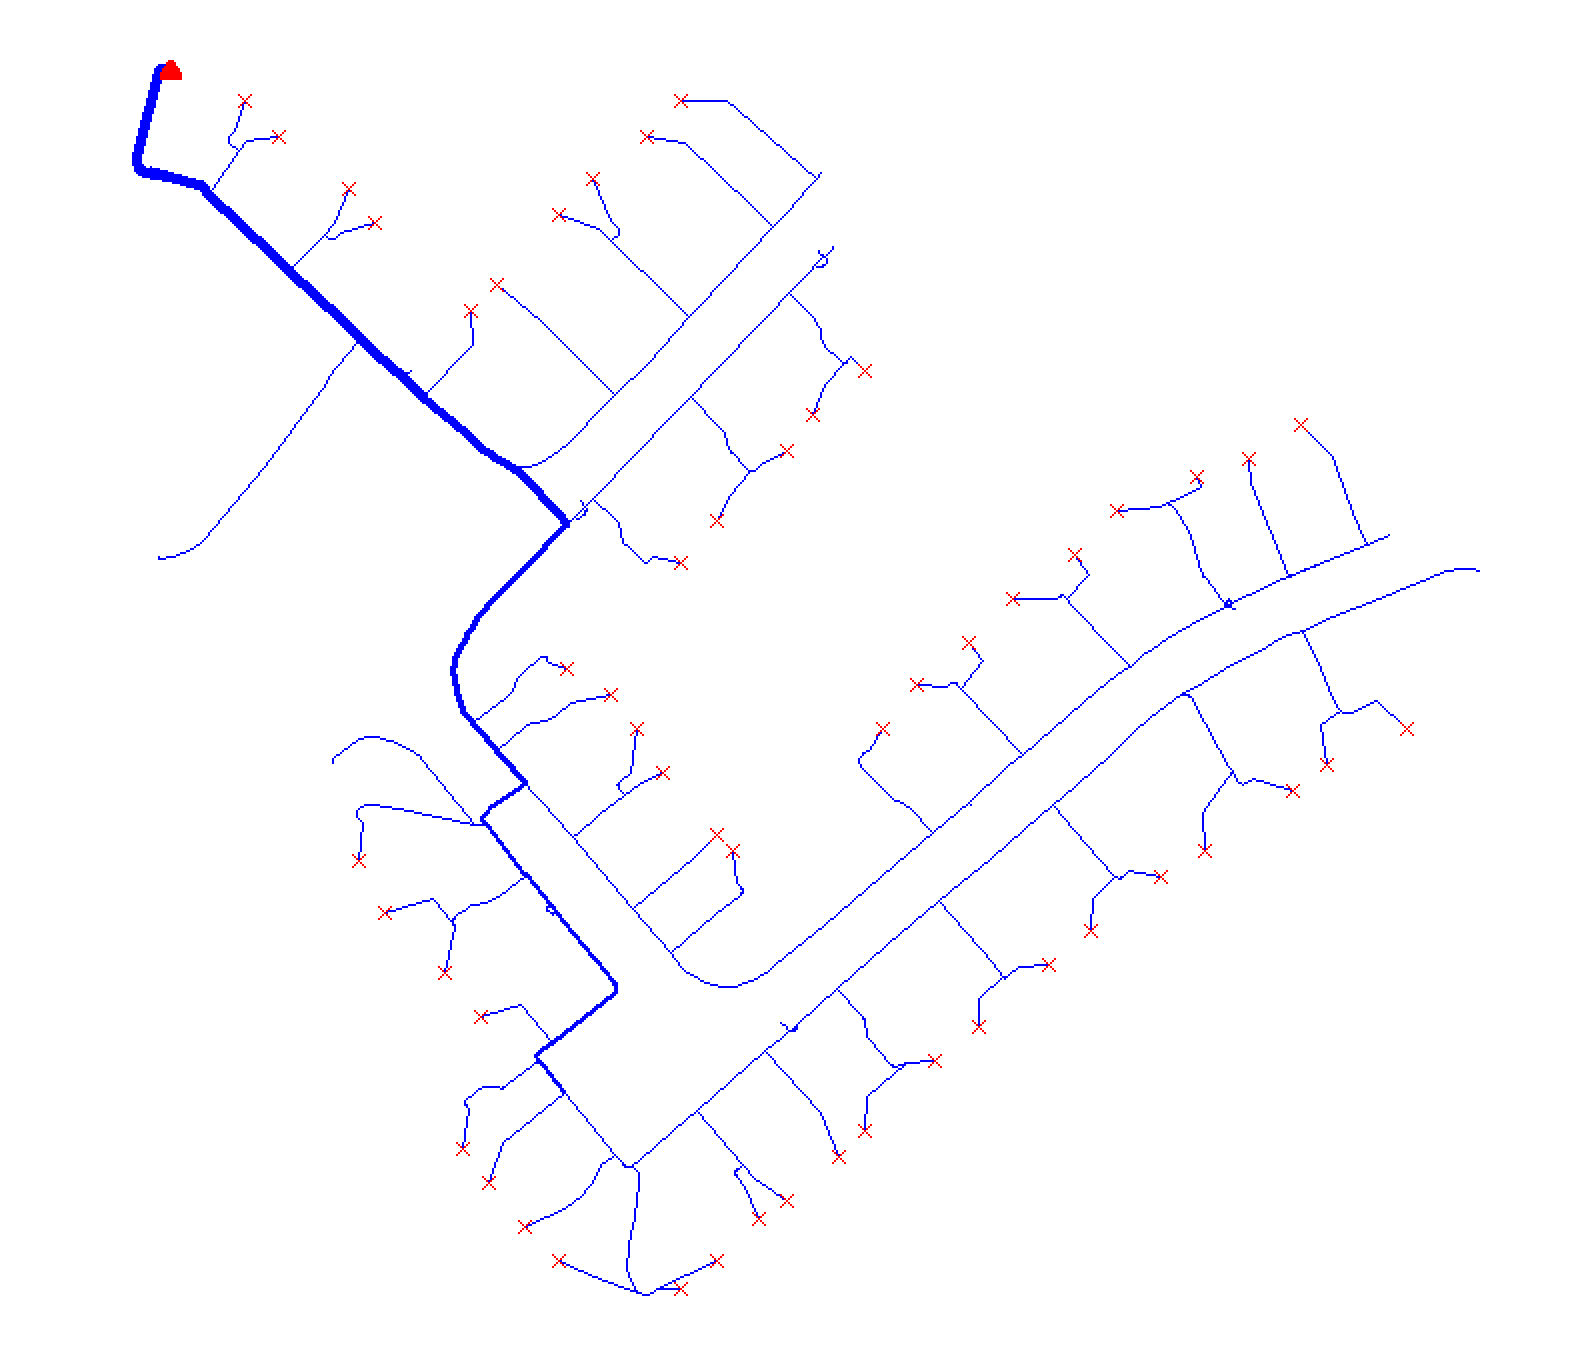
\includegraphics[width=0.8\textwidth]{_chapter1/fig/network-plot-LVTestCase}
	\caption{A power flow plot of the IEEE-PES European Test Case Feeder, i.e. a LV distribution network in the UK.}
	\label{ch1:fig:network-plot-LVTestCase}
\end{figure}

A substation (triangle in north west) provides power to the feeder, and the power magnitude is visualised by the thickness of the feeder's lines.
In total, there are 55 single-phase households connected to the substation, which represents a medium-sized, unbalanced UK feeder.

\subsection{Battery model}
\label{ch1:subsec:battery-model}

\nomenclature[I]{$S_\text{rating}$}{Rating of battery's power electronics, where $S_\text{rating} \in \mathbb{R}_{>0}$ (Chapter \ref{ch1})}

The ESMU systems that were deployed throughout the NTVV project consisted of two parts: the Power Management Unit (PMU) and the Energy Storage Unit (ESU).
The PMU controls three-phase powers and links the ESU to the grid.
Each PMU's single-phase power rating, $S_\text{rating}$, is 12kVA and can also perform filtering functions beside battery charging and discharging, e.g. compensating for harmonic distortion, reactive power and phase unbalance.
The ESU is a modular container of 12.5kWh of Li-Ion energy storage that can be aggregated to increase the total energy storage capacity.
All battery monitoring, conditioning and regulation is performed within the ESU and hence lies outside the scope of this work.
However, control instructions that are sent to the ESMU system should not request the device to operate outside its own specifications, i.e. avoid under- or over-charge.

\nomenclature[I]{$C_\text{bat}$}{Battery capacity, where $C_\text{bat} \in \mathbb{R}_{>0}$ (Chapter \ref{ch1})}
\nomenclature[I]{$E_\text{bat}(t)$}{Energy stored in battery at time $t$, where $E_\text{bat}(t) \in \mathbb{R}_{>0}$ (Chapter \ref{ch1})}
\nomenclature[I]{$\eta$}{Round-trip efficiency of power electronics, where $\eta \in (0, 1]$ (Chapter \ref{ch1})}
\nomenclature[I]{$p_\text{bat}(t)$}{Single-phase active battery power at time $t$, where $p_\text{bat}(t) \in \mathbb{R}$ (Chapter \ref{ch1})}
\nomenclature[I]{$s_{\text{ESMU},\phi}(t)$}{Single-phase apparent ESMU power for phase $\phi$ at time $t$, where $\textbf{s}_\text{ESMU}(t) = (s_{\text{ESMU},\phi}(t))$ and $s_{\text{ESMU},\phi}(t) \in \mathbb{C}$ (Chapter \ref{ch1})}
\nomenclature[I]{$\textbf{s}_\text{ESMU}(t)$}{Three-phase apparent ESMU power at time $t$, where $\textbf{s}_\text{ESMU}(t) = (s_{\text{ESMU},\phi}(t))$ and $\textbf{s}_\text{ESMU}(t) \in \mathbb{C}^{\Phi}$ (Chapter \ref{ch1})}

In order to simulate this ESMU system and its energy storing behaviour, a model is developed from the given device specifications.
This model includes an charge-discharge efficiency, $\eta$, and standby losses, $\mu$.
$\eta$ is related to the efficiency of the PMU's power converters, which are quoted to have a round trip efficiency of 98\%, i.e. $\eta = 0.98$.
$\mu$ on the other hand is linked to the nominal power drawn by the battery's control system as well as the battery's self-discharge rate.
With the charge-discharge efficiency, $\eta$, the battery charge-discharge power, $p_\text{bat}(t)$, can be calculated for any given ESMU power, $\textbf{s}_\text{ESMU}(t)$ (where $\textbf{s}_\text{ESMU}(t) = (s_{\text{ESMU},\phi}(t))$).

\begin{equation}
\begin{split}
	s_\text{bat}(t) = 
	\begin{cases}
		\eta\text{Re}\left\{\sum_{\phi=1}^{\Phi}s_{\text{ESMU},\phi}(t)\right\} &\text{ if } \text{Re}\left\{\sum_{\phi=1}^{\Phi}s_{\text{ESMU},\phi}(t)\right\} \geq 0\\
		\frac{1}{\eta}\text{Re}\left\{\sum_{\phi=1}^{\Phi}s_{\text{ESMU},\phi}(t)\right\} &\text{ otherwise}
	\end{cases} \forall t \\
	\text{and } \phi \in [1, \dots, \Phi] \text{ and } \Phi \in \mathbb{Z}^{>0}
\end{split}
\label{ch1:equ:battery-power-definition}
\end{equation}

\nomenclature[I]{$C_f$}{Charge factor or ``C-factor'' of the battery, where $C_f \in \mathbb{R}_{>0}$ (Chapter \ref{ch1})}

Although the ESMU's PSU rating, $S_\text{rating}$, may allow for a maximum power consumption of 36kVA (i.e. $=3\times12\text{kVA}$), the charging power is internally limited, by a charging factor, $C_f$.
This factor is the ratio between the battery's maximum discharge power and its total capacity (i.e. $\max_t (p_\text{bat}(t)) \leq C_f \cdot C_\text{bat}$).
In accordance to the ESMU's specification, $C_f$ was fixed as 1.6.
With those restrictions in mind, a charge-discharge power can be applied to charge or discharge the battery.
Assuming that this power remains constant during a predefined sample period, $\Delta t$, then the change in stored energy can be defined as follows.

\begin{equation}
	\Delta E_{battery}(t) = s_{battery}(t)t_s \forall t
	\label{ch1:equ:change-in-energy}
\end{equation}

\nomenclature[I]{$\mu$}{Self-discharge losses of battery, where $\mu \in (0, 1]$ (Chapter \ref{ch1})}
\nomenclature[I]{$\Delta E_\text{bat}(t)$}{Change in stored energy at time $t$, where $\Delta E_\text{bat}(t) \in \mathbb{R}$ (Chapter \ref{ch1})}
\nomenclature[I]{$SOC(t)$}{State of charge at time $t$, where $SOC(t) \in (0, 1)$ (Chapter \ref{ch1})}

The battery's dynamics can therefore be modelled as the change in energy level from time $t$ to time $t+\Delta t$.
Taking into account the standby losses, $\mu$, the next energy level $E_\text{bat}(t+\Delta t)$ is defined as:

\begin{equation}
	E_{battery}(t+1) = \mu\left(\Delta E_{battery}(t) + E_{battery}(t)\right)
\label{ch1:equ:next-energy}
\end{equation}

In an ideal case, $\mu = 1$, where no energy would be lost in the storage system.
However, to model energy storage dynamics, it became common practice to assess the energy storage's charge level as the State of Charge (SOC) instead of using the actual charge stored.
This SOC is defined as the actual energy stored in the ESU, $E_\text{bat}(t)$, divided by the total capacity of the system, $C_\text{bat}$. i.e.:

\begin{equation}
	SOC(t) := \frac{E_{battery}(t)}{C_{battery}} \forall t
	\label{ch1:equ:state-of-charge-definition}
\end{equation}

Similar to the energy dynamics, the SOC dynamics can therefore be defined as:

\begin{equation}
	SOC(t+\Delta t) := \mu\left(\frac{p_\text{bat}(t)\Delta t}{C_\text{bat}} + SOC(t)\right)
	\label{ch1:equ:next-state-of-charge}
\end{equation}

When summarising $\hat{s}_\text{ESMU}(t) = \text{Re}\left\{\sum_{\phi=1}^{\Phi}s_{\text{ESMU},\phi}(t)\right\}$ and combining Equation \ref{ch1:equ:battery-power-definition} with Equation \ref{ch1:equ:next-state-of-charge}, then the battery model's full dynamics can be defined as:

\begin{equation}
	SOC(t+\Delta t) := 
	\begin{cases}
		\mu\left(\frac{\eta \hat{s}_\text{ESMU}(t)\Delta t}{C_\text{bat}} + SOC(t)\right)	&\text{if } \hat{s}_\text{ESMU}(t) \geq 0\\
		\mu\left(\frac{\hat{s}_\text{ESMU}(t)\Delta t}{\eta C_\text{bat}} + SOC(t)\right) &\text{otherwise}
	\end{cases}
	\forall t
	\label{ch1:equ:next-state-of-charge-2}
\end{equation}

A flowchart to visually represent the developed battery model, is included in Figure \ref{ch1:fig:next-soc-flowchart}.
In this figure, all green and blue fields indicate, respectively, model inputs and results.
The white states represent operations applied onto those inputs and results and in the end yield the output, i.e. the yellow field.

\begin{figure}\centering
% Define some block styles
\tikzstyle{input} = [%
	draw,%
	ellipse,%
	fill=green!20,%
	minimum height=2em,%
]
\tikzstyle{result} = [%
	draw,%
	ellipse,%
	fill=blue!20,%
	minimum height=2em,%
]
\tikzstyle{output} = [%
	draw,%
	ellipse,%
	fill=yellow!20,%
	minimum height=2em,%
]
\tikzstyle{decision} = [%
	diamond,%
	draw,%
	text width=4.5em,%
	text badly centered,%
	inner sep=0pt%
]
\begin{tikzpicture}[node distance=3cm, shorten >= 1pt, >=stealth', auto]

	% Define nodes
    \node (power_esmu) [input] {$\textbf{s}_{ESMU}(t)$};
    \node (is_charging) [decision, right of=power_esmu] {charging\footnotemark[2]};
    \node (charging) [state, above right of=is_charging] {$\times\eta$};
    \node (discharging) [state, below right of=is_charging] {$\times\frac{1}{\eta}$};
    \node (power_battery) [result, below right of=charging] {$s_{battery}(t)$};
    \node (sample) [state, right of=power_battery] {$\times \tau$};
    \node (change_energy_battery) [result, below of=sample, yshift=5mm] {$\Delta E_{battery}(t)$};
    \node (add) [state, below of=change_energy_battery, yshift=5mm] {$+$};
    \node (current_energy_battery) [result, left of=add] {$E_{battery}(t)$};
    \node (multiply) [state, left of=current_energy_battery] {$\times C_{battery}$};
    \node (current_soc) [input, left of=multiply] {$SOC(t)$};
    \node (losses) [state, below of=add, yshift=5mm] {$\times \mu \tau$};
	\node (next_energy) [result, left of=losses, xshift=-5mm] {$E_{battery}(t+1)$};
	\node (divide) [state, left of=next_energy, xshift=-5mm] {$\div C_{battery}$};
	\node (next_soc) [output, left of=divide, xshift=-5mm] {$SOC(t+1)$};

	% Draw lines
	\draw [->] (power_esmu) to (is_charging);
	\draw [->, bend left] (is_charging) to node {yes} (charging);
	\draw [->, bend right] (is_charging) to node [swap] {no} (discharging);
	\draw [->, bend left] (charging) to (power_battery);
	\draw [->, bend right] (discharging) to (power_battery);
	\draw [->] (power_battery) to (sample);
	\draw [->] (sample) to (change_energy_battery);
	\draw [->] (change_energy_battery) to (add);
	\draw [->] (current_soc) to (multiply);
	\draw [->] (multiply) to (current_energy_battery);
	\draw [->] (current_energy_battery) to (add);
	\draw [->] (add) to (losses);
	\draw [->] (losses) to (next_energy);
	\draw [->] (next_energy) to (divide);
	\draw [->] (divide) to (next_soc);
	
\end{tikzpicture}
\caption{Flowchart to calculate the next SOC (i.e. $SOC(t+1)$) based on current ESMU power (i.e. $\textbf{s}_{ESMU}(t)$) and current SOC (i.e. $SOC(t)$)}
\end{figure}

\footnotetext[2]{In the flowchart ``charging'' implies that $\sum_{\phi=1}^{\Phi}s_{ESMU,\phi}(t) \geq 0$ as explained in Equation \ref{ch1:equ:battery-power-definition}.}

\subsection{ESMU scheduling}
\label{ch1:subsec:esmu-scheduling}

Computing the ESMU's daily schedule at the dataset's temporal resolution, i.e. sub-half-hourly, is ineffective and slow.
Doing so is ineffective, because demand variability due to behavioural unpredictability makes forecasting at high temporal resolution unfeasible, and the large number of search parameters makes finding a solutions very computationally demanding.
Therefore, forecasting and scheduling is generally performed at half-hourly temporal resolution.
To obtain such a half-hourly profile, the sub-half-hourly profile had to be down-sampled and synchronised.
This is done with the synchronisation function $k(t)$, which links the original sub-half-hourly demand to a half-hourly time-series and is defined as follows:

\begin{equation}
	k(t) := \left\lfloor\frac{t-1}{K\Delta t}\right\rfloor+1
	\label{ch1:equ:synchronisation-function}
\end{equation}

\nomenclature[I]{$K$}{Number of sample periods over which the sub-half-hourly is to be downsampled, where $K \in \mathbb{Z}_{>0}$ and $\frac{T_\text{sch}}{K} \in \mathbb{Z}_{>0}$ (Chapter \ref{ch1})}
\nomenclature[I]{$k(t)$}{Synchronisation function used to downsample the sub-half-hourly profile (Chapter \ref{ch1})}
\nomenclature[I]{$T_\text{sch}$}{Scheduling horizon, where $T_\text{sch} \in \mathbb{Z}_{>0}$ (Chapter \ref{ch1})}
\nomenclature[I]{$s^*_\text{net}(t)$}{Half-hourly network load, where $\textbf{s}^*_\text{net} = (s^*_\text{net}(t))$ and $s^*_\text{net}(t) \in \mathbb{C}$ (Chapter \ref{ch1})}
\nomenclature[I]{$\textbf{s}^*_\text{net}$}{Half-hourly network load, where $\textbf{s}^*_\text{net} \in \mathbb{C}^{\frac{T_\text{sch}}{K}}$ (Chapter \ref{ch1})}

Here, $\Delta t$ is the sub-half-hourly sampling period of the simulation, and $K$ is the duration of the half-hourly time-slot, i.e. number of sub-half-hourly periods within the half-hourly slot.
It should be noted that the integer multiple of $K$ has to equate to the scheduling horizon's length, $T_\text{sch}$; i.e. $a := \frac{K}{T_\text{sch}} \text{ where } a \in \mathbb{Z}_{>0}$.
Otherwise, the sub-half-hourly profile cannot be divided into a set of equal length time-slots, where each time-slot is of length $K\Delta t$.
Therefore, the resulting half-hourly network load, $s^{*}_\text{net}(t)$ (where $\textbf{s}^*_\text{net} = (s^*_\text{net}(t))$), is defined as follows:

\begin{equation}
	s^*_{network\;\;load}(t^*) = \frac{T^*}{T}\sum_{t=1}^{\frac{T}{T^*}}s_{network\;\;load}\left(\frac{T}{T^*}(t^*-1) + t\right) \forall t^* \text{ where } t^* \in [1, \dots, T^{*}]
	\label{ch1:equ:down-sampling-to-half-hourly}
\end{equation}

Now, over the period from $\alpha(t)$ to $\beta(t)$, are power values are equal.
To illustrate the difference between the original sub-half-hourly network load and the resulting half-hourly demand, both profiles are plotted in Figure \ref{ch1:fig:sub-half-horuly-demand-comparison}.
In this figure, it can be observed how the high variability and volatility in power is removed in the half-hourly profile.
When generating ESMU schedules these variations are neglected and thus the unwanted peak power demands cannot be sufficiently compensated.

\begin{figure}\centering
	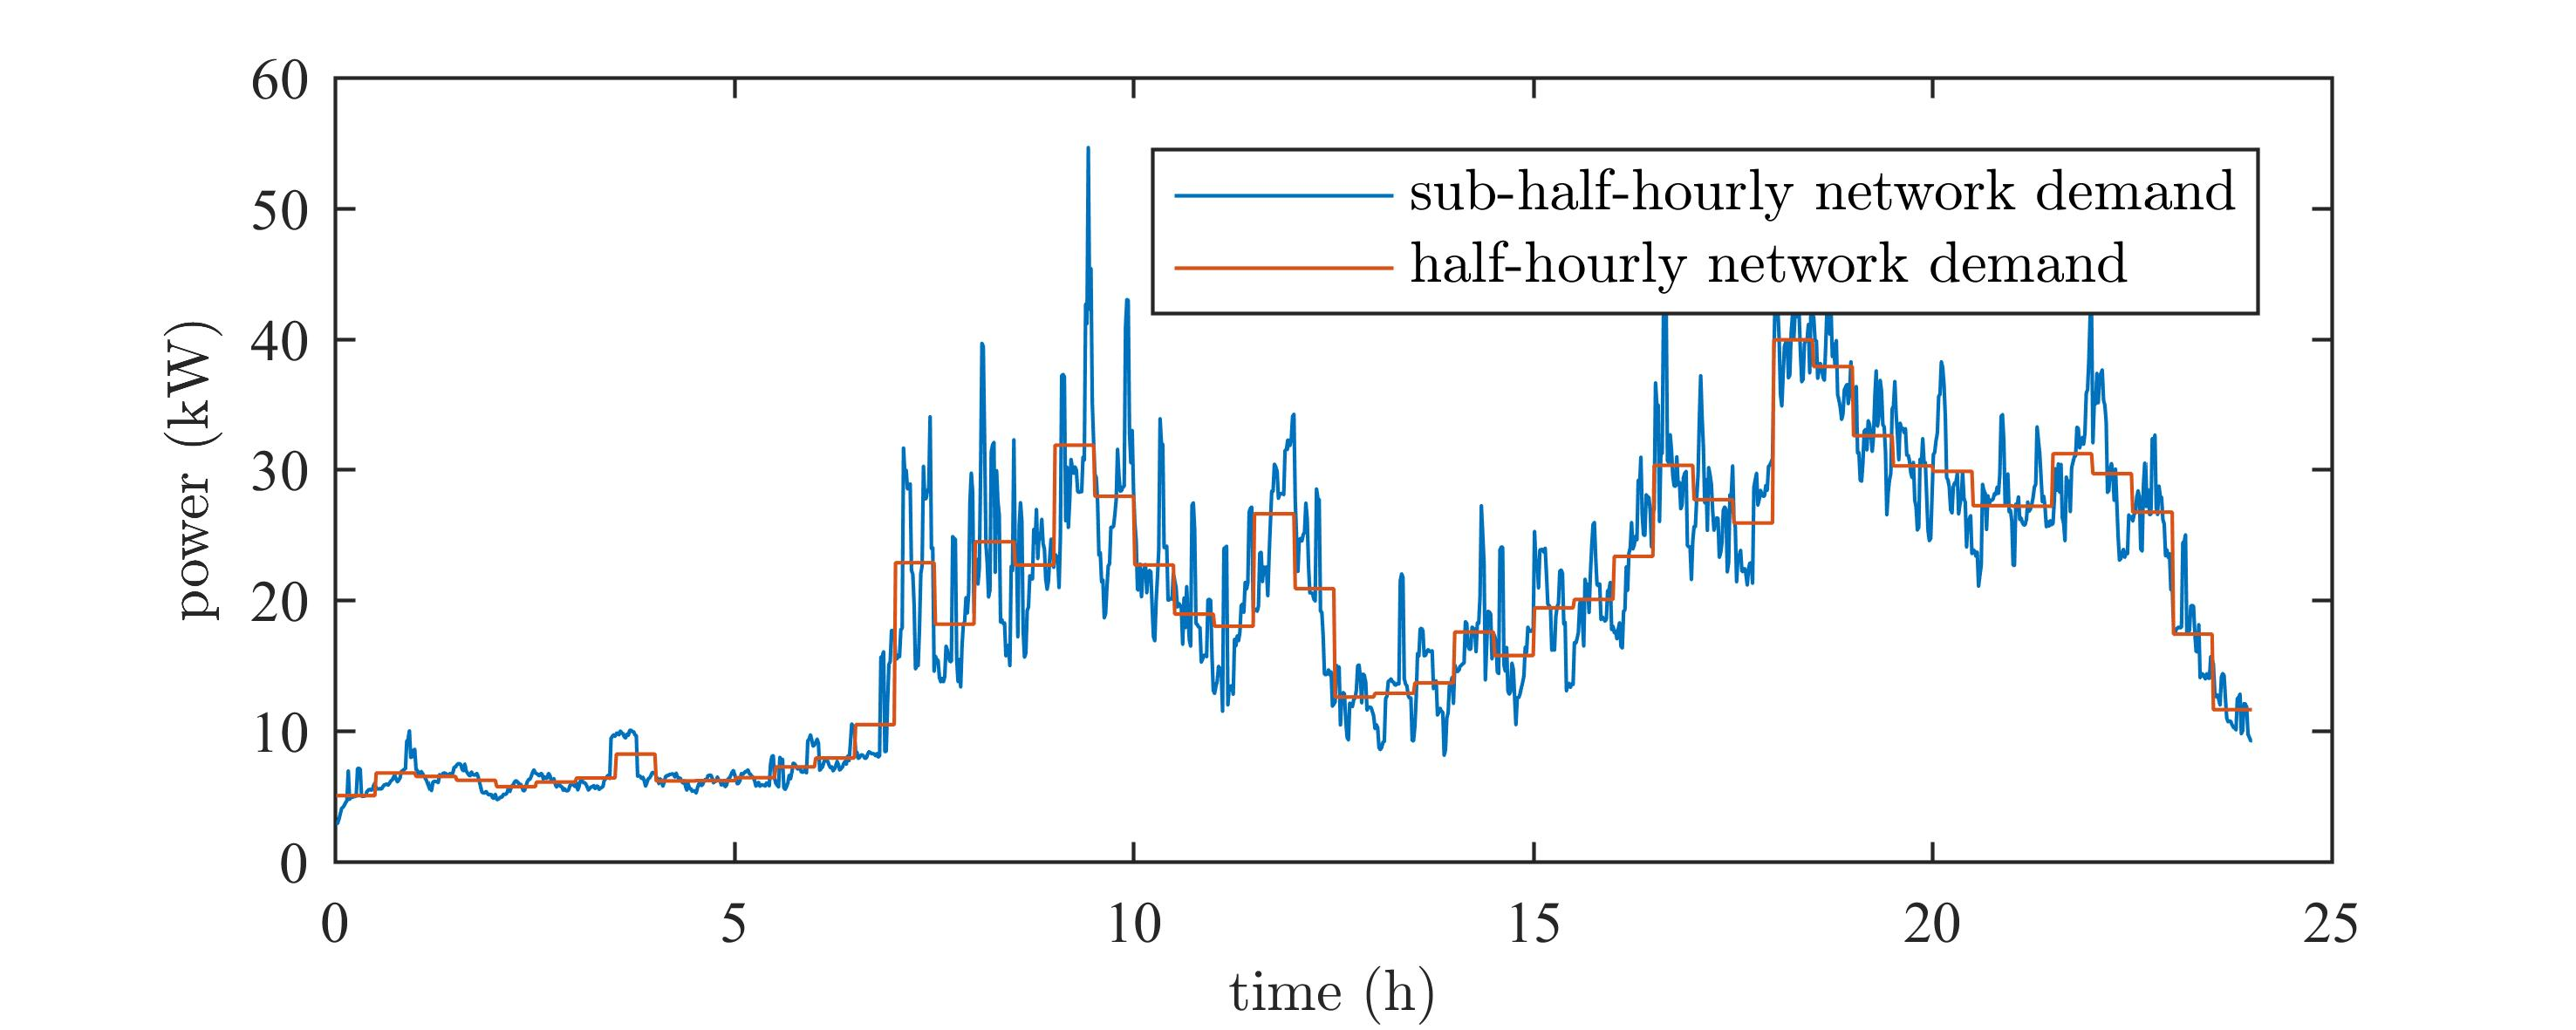
\includegraphics{_chapter1/fig/sub-half-horuly-demand-comparison}
	\caption{Highly variable and volatile demand profile vs half-hourly demand (i.e. a forecast under perfect foresight conditions)}
	\label{ch1:fig:sub-half-horuly-demand-comparison}
\end{figure}

The main goals when scheduling battery operation are to achieve ``valley-filling'' and ``peak-shaving'' behaviour.
As shown in the literature review in Chapter \ref{ch-review}, the Peak-to-Average Ratio (PAR), the min-max-difference (MMD) and the power transients (TRA) are good indicators of such a behaviour.
Therefore, three half-hourly costs regarding are used as, $\zeta_\text{PAR}(\textbf{s}^*_\text{ESMU} + \textbf{s}^*_\text{net})$, $\zeta_\text{MMD}(\textbf{s}^*_\text{ESMU} + \textbf{s}^*_\text{net})$, and $\zeta_\text{TRA}(\textbf{s}^*_\text{ESMU} + \textbf{s}^*_\text{net})$ are defined as follows:

\begin{equation}
\begin{split}
	\zeta_{PAR}(\textbf{s}_{A}, \textbf{s}_{B}) :=& \frac{\max_k \left| \textbf{s}_{A}+\textbf{s}_{B}\right|}{\frac{1}{K}\sum_{k=1}^{K}\left[{s}_{A}(k)+{s}_{B}(k)\right]} - 1\\
	& \text{where } {s}_{A}(k) \in \textbf{s}_{A} \text{ and } {s}_{B}(tk \in \textbf{s}_{B}
\end{split}
\label{ch1:equ:peak-to-average-definition}
\end{equation}

\begin{equation}
	\zeta_\text{MMD}(\textbf{s}) := \frac{\max_k \left(\textbf{s}\right) - \min_k\left(\textbf{s}\right)}{\frac{1}{K}\sum_{t=1}^{\frac{T_\text{sch}}{K}}s(t)}
	\text{ where } (s(t)) = \textbf{s}
\label{ch1:equ:min-max-difference-definition}
\end{equation}

\begin{equation}
	\zeta_\text{TRA}(\textbf{s}) := \max_t \left|s(t + \Delta t) - s(t) \right|
	\text{ where } ({s}(t)) = \textbf{s}
\label{ch1:equ:power-transients-definition}
\end{equation}

\nomenclature[I]{$\zeta_\text{PAR}(\textbf{s})$}{Cost of the underlying power profile $\textbf{s}$, based on the Peak to Average Ratio (PAR), where $\zeta_\text{PAR}(\textbf{s}) \in \mathbb{R}_{\geq0}$ (Chapter \ref{ch1})}
\nomenclature[I]{$\zeta_\text{MMD}(\textbf{s})$}{Cost of the underlying power profile $\textbf{s}$, based on the Minimum-Maximum Difference (MMD), where $\zeta_\text{MMD}(\textbf{s}) \in \mathbb{R}_{\geq0}$ (Chapter \ref{ch1})}
\nomenclature[I]{$\zeta_\text{TRA}(\textbf{s})$}{Cost of the underlying power profile $\textbf{s}$, based on the power transients (TRA), where $\zeta_\text{MMD}(\textbf{s}) \in \mathbb{R}_{\geq0}$ (Chapter \ref{ch1})}

All three costs functions assess the sum of the half-hourly ESMU schedule, $\textbf{s}^*_\text{ESMU}$, and the half-hourly network load profile, $\textbf{s}^*_\text{net}$.
Combined with all underlying model constraints, the following minimisation problem is defined:

\begin{equation}
\begin{split}
	\min_{\textbf{s}^*_\text{ESMU}} & \left\{\zeta_\text{PAR}(\textbf{s}^*_\text{ESMU}, \textbf{s}^*_\text{net}) + \zeta_\text{MMD}(\textbf{s}^*_\text{ESMU}, \textbf{s}^*_\text{net}) + \zeta_\text{TRA}(\textbf{s}^*_\text{ESMU}, \textbf{s}^*_\text{net})\right\}\\
	\text{s.t. }& \begin{cases}
		p_\text{bat}(t) \leq C_f\times C_\text{bat}\\
		\left|s_{\text{ESMU},\phi}(t)\right| \leq S_\text{rating} \forall \phi\\
		0 \leq SOC(t) \leq 1
	\end{cases}
\end{split}
\label{ch1:equ:scheduling-cost}
\end{equation}

For this piece of work, a Sequential Quadratic Programming (SQP) approach was chosen to solve this minimisation problem.
The resulting half-hourly ESMU power, $\textbf{s}^*_\text{ESMU}$, could then be extrapolated using the same synchronisation function, $k(t)$, to yield a sub-half-hourly ESMU schedule.

For the work presented in this chapter, the supplied half-hourly network load (or forecast) was obtained from sub-half-hourly data.
Treating it as a forecast with perfect foresight does not skew the already imperfect schedule performance, which is obtained when applying the resulting half-hourly schedule to sub-half-hourly load.
Figure \ref{ch1:fig:improved-network-power} shows a sample day, where the impact of this half-hourly ESMU schedule becomes apparent.

\begin{figure}\centering
	\subfloat[Half-hourly ESMU power impact ($\Delta S = 9.46kW$)]{%
		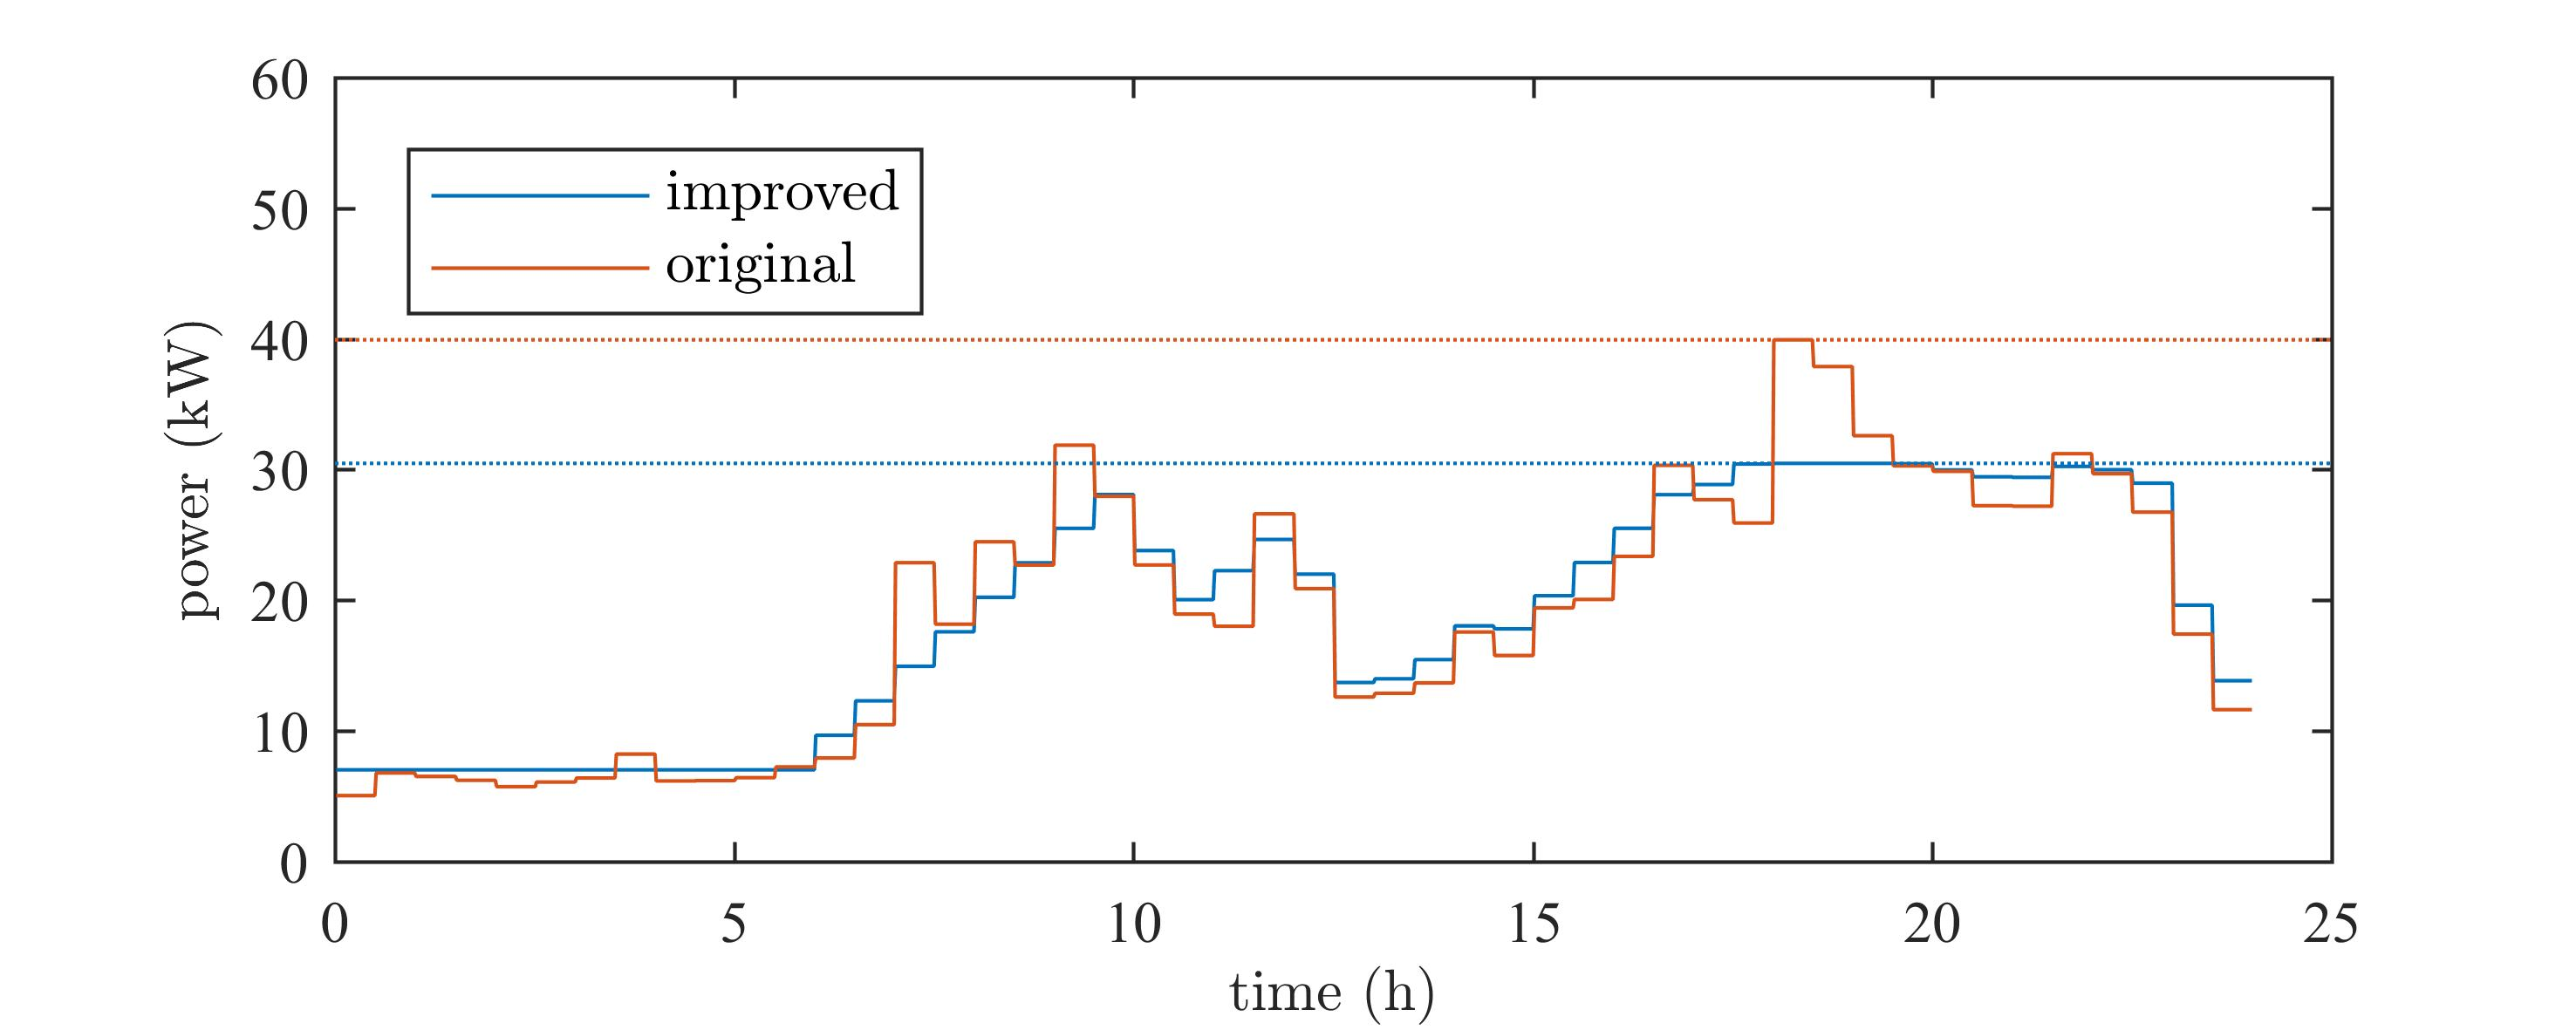
\includegraphics{_chapter1/fig/improved-half-hourly-network-power}%
		\label{ch1:subfig:improved-half-hourly-network-power}%
	}
	\vspace{5mm}
	\subfloat[Sub-half-hourly ESMU power impact ($\Delta S = 6.36kW$)]{%
		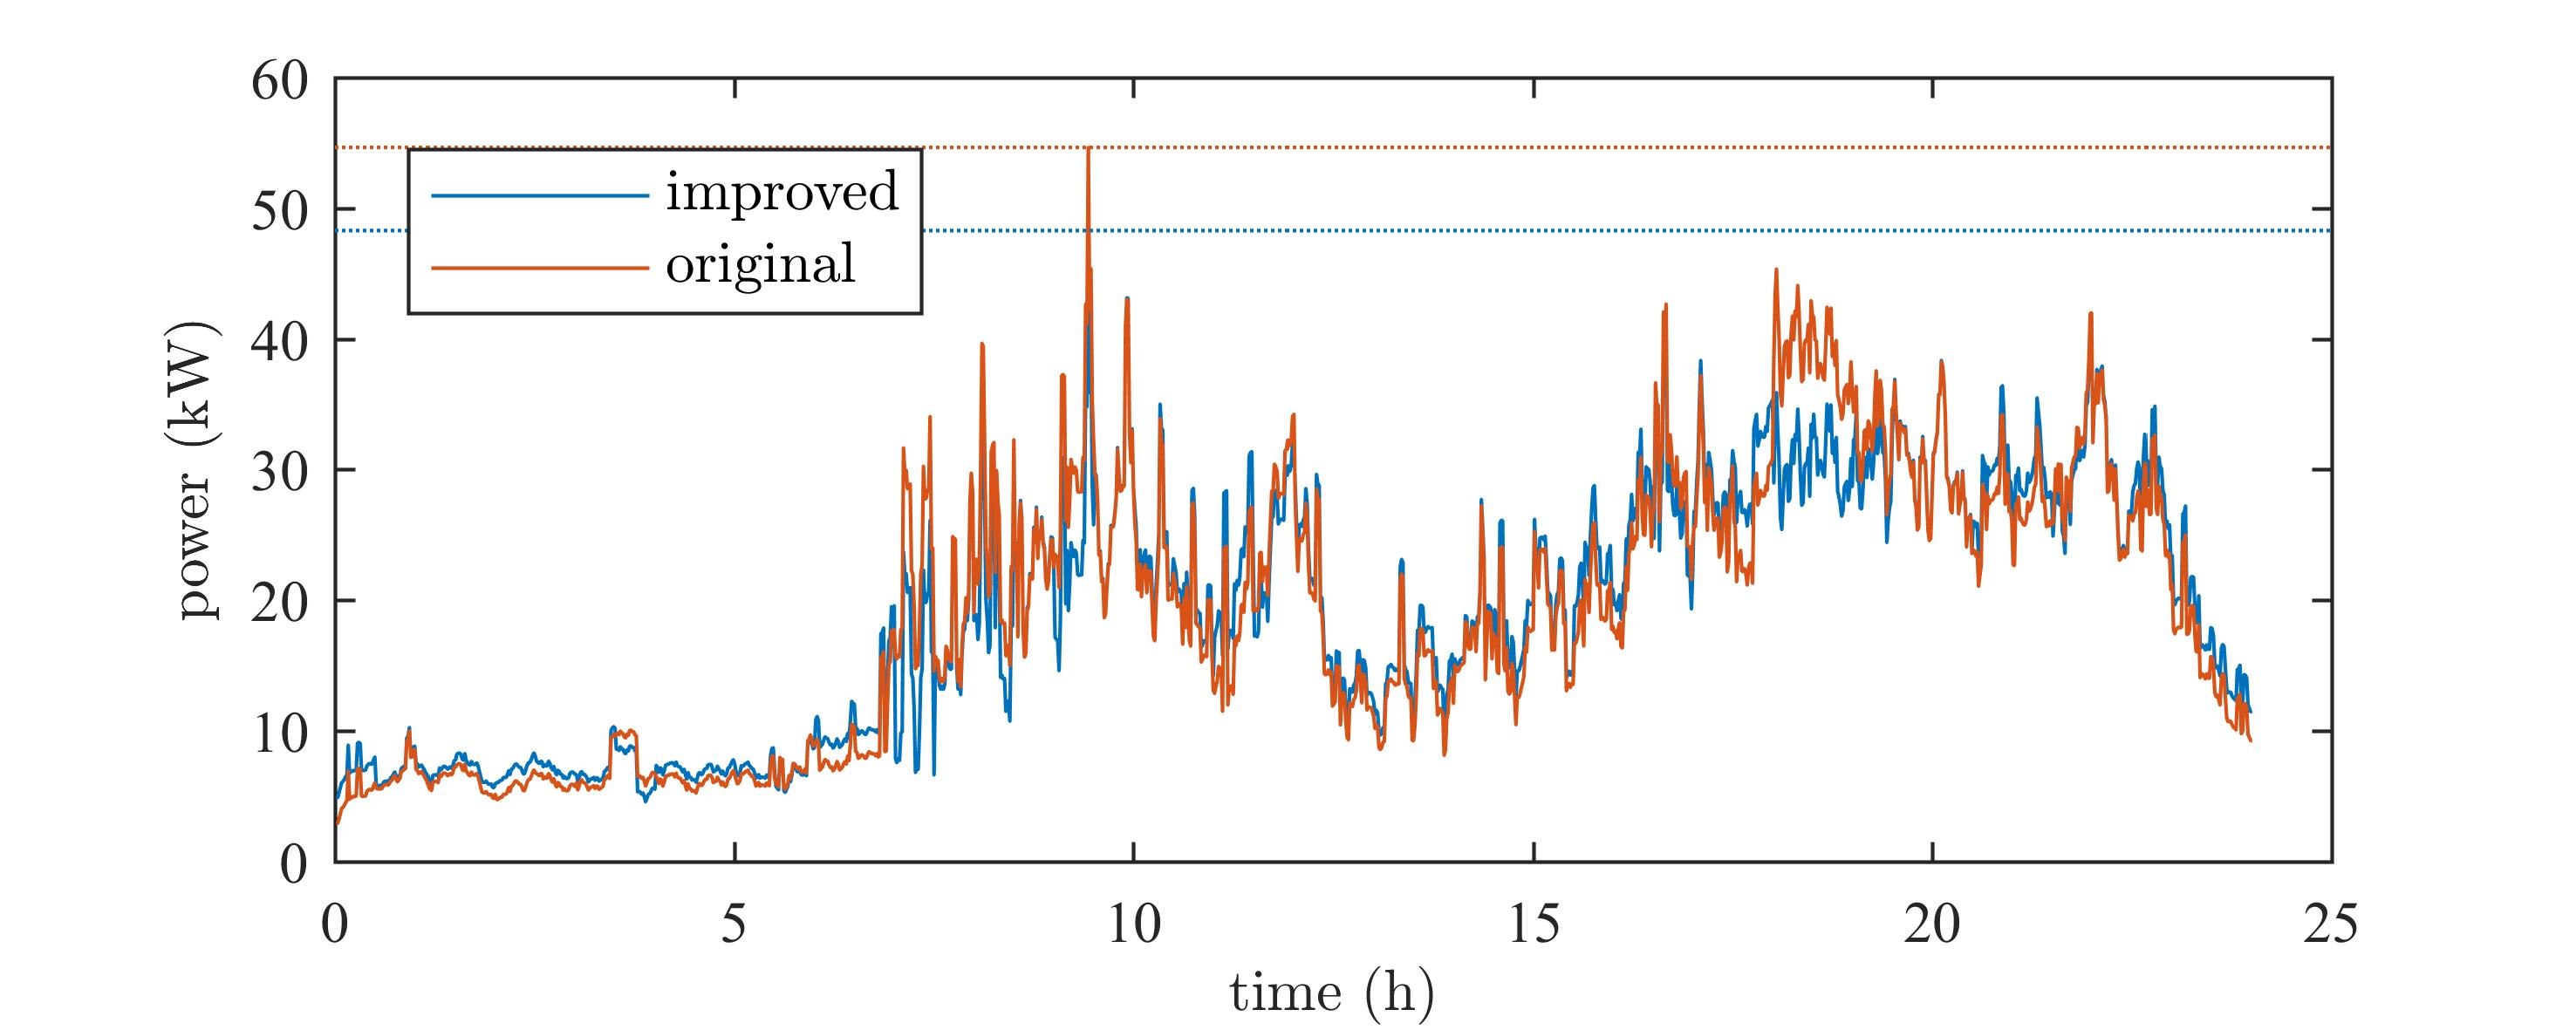
\includegraphics{_chapter1/fig/improved-sub-half-hourly-network-power}%
		\label{ch1:subfig:improved-sub-half-hourly-network-power}%
	}
	\caption{Impact of half-hourly ESMU schedule on sub-half-hourly power profile}
	\label{ch1:fig:improved-network-power}
\end{figure}

This figure shows the positive impact on the half-hourly profile (i.e. in Figure \ref{ch1:subfig:improved-half-hourly-network-power}), which is particularly dominant during the evening peak load.
However, the impact on the actual sub-half-hourly demand (i.e. in Figure \ref{ch1:subfig:improved-sub-half-hourly-network-power}) has a much larger demand spike during the morning hours, which is not that strongly addressed.
When compared, the ideal peak power shaving dropped from 9.46kW to only 6.36kW.
Nonetheless, the overall improvement yielded by the ESMU schedule can still be noticed. 
The method of how to adjust the ESMU's phase powers to mitigate the impact of such volatile load spikes is addressed in the following section.

